\documentclass[]{article}
\usepackage{lmodern}
\usepackage{amssymb,amsmath}
\usepackage{ifxetex,ifluatex}
\usepackage{fixltx2e} % provides \textsubscript
\ifnum 0\ifxetex 1\fi\ifluatex 1\fi=0 % if pdftex
  \usepackage[T1]{fontenc}
  \usepackage[utf8]{inputenc}
\else % if luatex or xelatex
  \ifxetex
    \usepackage{mathspec}
  \else
    \usepackage{fontspec}
  \fi
  \defaultfontfeatures{Ligatures=TeX,Scale=MatchLowercase}
\fi
% use upquote if available, for straight quotes in verbatim environments
\IfFileExists{upquote.sty}{\usepackage{upquote}}{}
% use microtype if available
\IfFileExists{microtype.sty}{%
\usepackage{microtype}
\UseMicrotypeSet[protrusion]{basicmath} % disable protrusion for tt fonts
}{}
\usepackage[margin=1in]{geometry}
\usepackage{hyperref}
\hypersetup{unicode=true,
            pdftitle={Locker-Angelina-ADA-Homework-02},
            pdfauthor={Angelina Locker},
            pdfborder={0 0 0},
            breaklinks=true}
\urlstyle{same}  % don't use monospace font for urls
\usepackage{color}
\usepackage{fancyvrb}
\newcommand{\VerbBar}{|}
\newcommand{\VERB}{\Verb[commandchars=\\\{\}]}
\DefineVerbatimEnvironment{Highlighting}{Verbatim}{commandchars=\\\{\}}
% Add ',fontsize=\small' for more characters per line
\usepackage{framed}
\definecolor{shadecolor}{RGB}{248,248,248}
\newenvironment{Shaded}{\begin{snugshade}}{\end{snugshade}}
\newcommand{\KeywordTok}[1]{\textcolor[rgb]{0.13,0.29,0.53}{\textbf{#1}}}
\newcommand{\DataTypeTok}[1]{\textcolor[rgb]{0.13,0.29,0.53}{#1}}
\newcommand{\DecValTok}[1]{\textcolor[rgb]{0.00,0.00,0.81}{#1}}
\newcommand{\BaseNTok}[1]{\textcolor[rgb]{0.00,0.00,0.81}{#1}}
\newcommand{\FloatTok}[1]{\textcolor[rgb]{0.00,0.00,0.81}{#1}}
\newcommand{\ConstantTok}[1]{\textcolor[rgb]{0.00,0.00,0.00}{#1}}
\newcommand{\CharTok}[1]{\textcolor[rgb]{0.31,0.60,0.02}{#1}}
\newcommand{\SpecialCharTok}[1]{\textcolor[rgb]{0.00,0.00,0.00}{#1}}
\newcommand{\StringTok}[1]{\textcolor[rgb]{0.31,0.60,0.02}{#1}}
\newcommand{\VerbatimStringTok}[1]{\textcolor[rgb]{0.31,0.60,0.02}{#1}}
\newcommand{\SpecialStringTok}[1]{\textcolor[rgb]{0.31,0.60,0.02}{#1}}
\newcommand{\ImportTok}[1]{#1}
\newcommand{\CommentTok}[1]{\textcolor[rgb]{0.56,0.35,0.01}{\textit{#1}}}
\newcommand{\DocumentationTok}[1]{\textcolor[rgb]{0.56,0.35,0.01}{\textbf{\textit{#1}}}}
\newcommand{\AnnotationTok}[1]{\textcolor[rgb]{0.56,0.35,0.01}{\textbf{\textit{#1}}}}
\newcommand{\CommentVarTok}[1]{\textcolor[rgb]{0.56,0.35,0.01}{\textbf{\textit{#1}}}}
\newcommand{\OtherTok}[1]{\textcolor[rgb]{0.56,0.35,0.01}{#1}}
\newcommand{\FunctionTok}[1]{\textcolor[rgb]{0.00,0.00,0.00}{#1}}
\newcommand{\VariableTok}[1]{\textcolor[rgb]{0.00,0.00,0.00}{#1}}
\newcommand{\ControlFlowTok}[1]{\textcolor[rgb]{0.13,0.29,0.53}{\textbf{#1}}}
\newcommand{\OperatorTok}[1]{\textcolor[rgb]{0.81,0.36,0.00}{\textbf{#1}}}
\newcommand{\BuiltInTok}[1]{#1}
\newcommand{\ExtensionTok}[1]{#1}
\newcommand{\PreprocessorTok}[1]{\textcolor[rgb]{0.56,0.35,0.01}{\textit{#1}}}
\newcommand{\AttributeTok}[1]{\textcolor[rgb]{0.77,0.63,0.00}{#1}}
\newcommand{\RegionMarkerTok}[1]{#1}
\newcommand{\InformationTok}[1]{\textcolor[rgb]{0.56,0.35,0.01}{\textbf{\textit{#1}}}}
\newcommand{\WarningTok}[1]{\textcolor[rgb]{0.56,0.35,0.01}{\textbf{\textit{#1}}}}
\newcommand{\AlertTok}[1]{\textcolor[rgb]{0.94,0.16,0.16}{#1}}
\newcommand{\ErrorTok}[1]{\textcolor[rgb]{0.64,0.00,0.00}{\textbf{#1}}}
\newcommand{\NormalTok}[1]{#1}
\usepackage{graphicx,grffile}
\makeatletter
\def\maxwidth{\ifdim\Gin@nat@width>\linewidth\linewidth\else\Gin@nat@width\fi}
\def\maxheight{\ifdim\Gin@nat@height>\textheight\textheight\else\Gin@nat@height\fi}
\makeatother
% Scale images if necessary, so that they will not overflow the page
% margins by default, and it is still possible to overwrite the defaults
% using explicit options in \includegraphics[width, height, ...]{}
\setkeys{Gin}{width=\maxwidth,height=\maxheight,keepaspectratio}
\IfFileExists{parskip.sty}{%
\usepackage{parskip}
}{% else
\setlength{\parindent}{0pt}
\setlength{\parskip}{6pt plus 2pt minus 1pt}
}
\setlength{\emergencystretch}{3em}  % prevent overfull lines
\providecommand{\tightlist}{%
  \setlength{\itemsep}{0pt}\setlength{\parskip}{0pt}}
\setcounter{secnumdepth}{0}
% Redefines (sub)paragraphs to behave more like sections
\ifx\paragraph\undefined\else
\let\oldparagraph\paragraph
\renewcommand{\paragraph}[1]{\oldparagraph{#1}\mbox{}}
\fi
\ifx\subparagraph\undefined\else
\let\oldsubparagraph\subparagraph
\renewcommand{\subparagraph}[1]{\oldsubparagraph{#1}\mbox{}}
\fi

%%% Use protect on footnotes to avoid problems with footnotes in titles
\let\rmarkdownfootnote\footnote%
\def\footnote{\protect\rmarkdownfootnote}

%%% Change title format to be more compact
\usepackage{titling}

% Create subtitle command for use in maketitle
\newcommand{\subtitle}[1]{
  \posttitle{
    \begin{center}\large#1\end{center}
    }
}

\setlength{\droptitle}{-2em}

  \title{Locker-Angelina-ADA-Homework-02}
    \pretitle{\vspace{\droptitle}\centering\huge}
  \posttitle{\par}
    \author{Angelina Locker}
    \preauthor{\centering\large\emph}
  \postauthor{\par}
      \predate{\centering\large\emph}
  \postdate{\par}
    \date{February 27, 2019}


\begin{document}
\maketitle

\subsection{R Markdown}\label{r-markdown}

This is an R Markdown document. Markdown is a simple formatting syntax
for authoring HTML, PDF, and MS Word documents. For more details on
using R Markdown see \url{http://rmarkdown.rstudio.com}.

When you click the \textbf{Knit} button a document will be generated
that includes both content as well as the output of any embedded R code
chunks within the document. You can embed an R code chunk like this:

\begin{Shaded}
\begin{Highlighting}[]
\KeywordTok{summary}\NormalTok{(cars)}
\end{Highlighting}
\end{Shaded}

\begin{verbatim}
##      speed           dist       
##  Min.   : 4.0   Min.   :  2.00  
##  1st Qu.:12.0   1st Qu.: 26.00  
##  Median :15.0   Median : 36.00  
##  Mean   :15.4   Mean   : 42.98  
##  3rd Qu.:19.0   3rd Qu.: 56.00  
##  Max.   :25.0   Max.   :120.00
\end{verbatim}

\subsection{Including Plots}\label{including-plots}

You can also embed plots, for example:

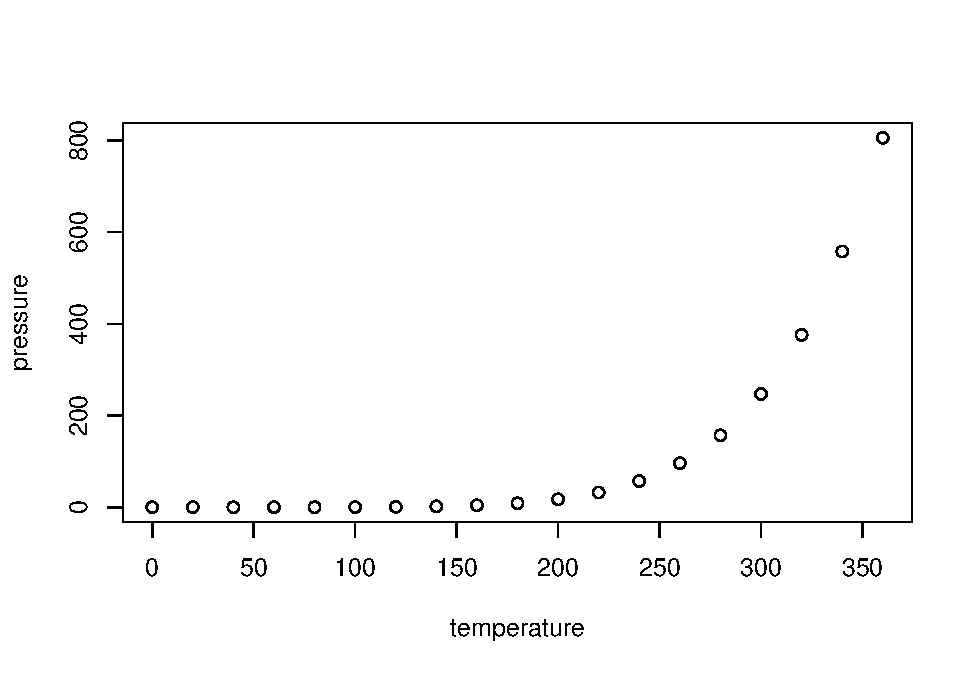
\includegraphics{Locker-Angelina-ADA-Homework-02_files/figure-latex/pressure-1.pdf}

Note that the \texttt{echo\ =\ FALSE} parameter was added to the code
chunk to prevent printing of the R code that generated the plot.

\begin{enumerate}
\def\labelenumi{\arabic{enumi}.}
\tightlist
\item
  Every Saturday, at the same time, a primatologist goes and sits in the
  forest in the morning and listens for titi monkey calls, counting the
  number of calls they hear in a 2 hour window from 5am to 7am. Based on
  previous knowledge, she believes that the mean number calls she will
  hear in that time is 15. Let X represent the appropriate Poisson
  random variable of the number of calls heard in each monitoring
  session.
\end{enumerate}

\begin{Shaded}
\begin{Highlighting}[]
\NormalTok{x <-}\StringTok{ }\DecValTok{0}\OperatorTok{:}\DecValTok{30}
\end{Highlighting}
\end{Shaded}

1.a. What is the probability that she will hear more than 8 calls during
any given session?

\begin{Shaded}
\begin{Highlighting}[]
\NormalTok{x <-}\StringTok{ }\DecValTok{0}\OperatorTok{:}\DecValTok{30}
\NormalTok{l <-}\StringTok{ }\DecValTok{15}
\NormalTok{a <-}\StringTok{ }\KeywordTok{ppois}\NormalTok{(}\DataTypeTok{q =} \DecValTok{8}\NormalTok{, }\DataTypeTok{lambda =} \DecValTok{15}\NormalTok{)}
\NormalTok{eightplus <-}\StringTok{ }\DecValTok{1}\OperatorTok{-}\NormalTok{a}
\NormalTok{eightplus}
\end{Highlighting}
\end{Shaded}

\begin{verbatim}
## [1] 0.9625535
\end{verbatim}

1.b. What is the probability that she will hear no calls in a session?

\begin{Shaded}
\begin{Highlighting}[]
\NormalTok{x <-}\StringTok{ }\DecValTok{0}\OperatorTok{:}\DecValTok{30}
\NormalTok{l <-}\StringTok{ }\DecValTok{15}
\NormalTok{b <-}\StringTok{ }\KeywordTok{ppois}\NormalTok{(}\DataTypeTok{q =} \DecValTok{0}\NormalTok{, }\DataTypeTok{lambda =} \DecValTok{15}\NormalTok{)}
\NormalTok{zero <-}\StringTok{ }\DecValTok{1}\OperatorTok{-}\NormalTok{b}
\NormalTok{zero}
\end{Highlighting}
\end{Shaded}

\begin{verbatim}
## [1] 0.9999997
\end{verbatim}

1.c. What is the probability that she will hear exactly 3 calls in a
session?

\begin{Shaded}
\begin{Highlighting}[]
\NormalTok{x <-}\StringTok{ }\DecValTok{0}\OperatorTok{:}\DecValTok{30}
\NormalTok{l <-}\StringTok{ }\DecValTok{15}
\NormalTok{c <-}\StringTok{ }\KeywordTok{dpois}\NormalTok{(}\DataTypeTok{x =} \DecValTok{3}\NormalTok{, }\DataTypeTok{lambda =} \DecValTok{15}\NormalTok{)}
\NormalTok{exactthree <-}\StringTok{ }\DecValTok{1}\OperatorTok{-}\NormalTok{c}
\NormalTok{exactthree}
\end{Highlighting}
\end{Shaded}

\begin{verbatim}
## [1] 0.9998279
\end{verbatim}

1.d. Plot the relevant Poisson mass function over the values in range 0
≤ x ≤ 30.

\begin{Shaded}
\begin{Highlighting}[]
\NormalTok{x <-}\StringTok{ }\DecValTok{0}\OperatorTok{:}\DecValTok{30}
\NormalTok{l <-}\StringTok{ }\DecValTok{15}
\NormalTok{probset <-}\StringTok{ }\KeywordTok{dpois}\NormalTok{(}\DataTypeTok{x =}\NormalTok{ x, }\DataTypeTok{lambda =}\NormalTok{ l)}
\KeywordTok{barplot}\NormalTok{(probset, }\DataTypeTok{names.arg =}\NormalTok{ x, }\DataTypeTok{space =} \DecValTok{0}\NormalTok{, }\DataTypeTok{xlab =} \StringTok{"x"}\NormalTok{, }\DataTypeTok{ylab =} \StringTok{"Pr(X = x)"}\NormalTok{, }\DataTypeTok{main =} \KeywordTok{paste0}\NormalTok{(}\StringTok{"Probability Mass Function}\CharTok{\textbackslash{}n}\StringTok{lambda = "}\NormalTok{, }\DecValTok{15}\NormalTok{))}
\end{Highlighting}
\end{Shaded}

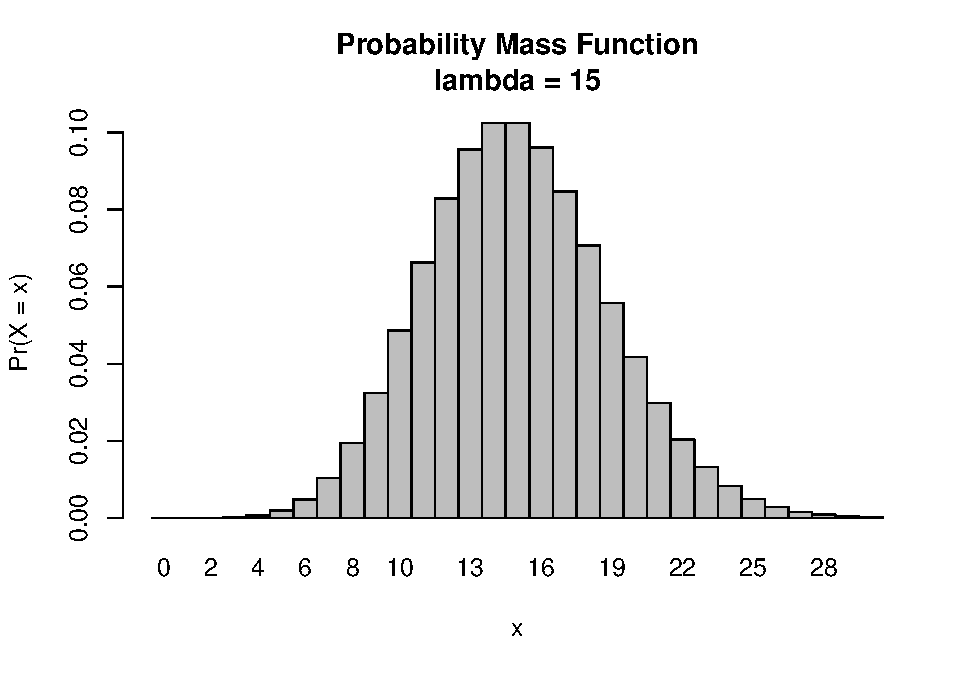
\includegraphics{Locker-Angelina-ADA-Homework-02_files/figure-latex/unnamed-chunk-5-1.pdf}

1.e. Simulate 104 results from this distribution (i.e., 2 years of
Saturday monitoring sessions).

\begin{Shaded}
\begin{Highlighting}[]
\NormalTok{x <-}\StringTok{ }\DecValTok{0}\OperatorTok{:}\DecValTok{30}
\NormalTok{l <-}\StringTok{ }\DecValTok{15}

\NormalTok{two_year <-}\StringTok{ }\KeywordTok{rpois}\NormalTok{(}\DataTypeTok{n =} \DecValTok{104}\NormalTok{, }\DataTypeTok{lambda =} \DecValTok{15}\NormalTok{)}


\NormalTok{two_year}
\end{Highlighting}
\end{Shaded}

\begin{verbatim}
##   [1] 23 12 20 18 12 23  9 12 19 12 19 17 17 14 14 19 12 14 12 14 14 14 13
##  [24] 14 11 16 15 21 14 18 14  5 10 19 18 17 13 19 18 12 10 14 16 15 11 18
##  [47] 12 11 14 11 14 11 20 15 15 15 13 21 16 19 13 11 14 16 15 21 13 20 14
##  [70] 19 23 15 17  9 17 17  9 16 17 20 14 19 17 17 16 16 17 18 14 11 20 15
##  [93]  9 16 12 12 15 12 23 16 14 18 16 17
\end{verbatim}

1.f. Plot the simulated results using hist() and use xlim() to set the
horizontal limits to be from 0 to 30. How does your histogram compare to
the shape of the probability mass function you plotted above?

\begin{Shaded}
\begin{Highlighting}[]
\NormalTok{two_year <-}\StringTok{ }\KeywordTok{rpois}\NormalTok{(}\DataTypeTok{n =} \DecValTok{104}\NormalTok{, }\DataTypeTok{lambda =} \DecValTok{15}\NormalTok{)}

\KeywordTok{hist}\NormalTok{(two_year, }\DataTypeTok{xlim=}\KeywordTok{c}\NormalTok{(}\DecValTok{0}\NormalTok{,}\DecValTok{30}\NormalTok{), }\DataTypeTok{xlab =} \StringTok{"Observation"}\NormalTok{, }\DataTypeTok{ylab =} \StringTok{"# of Calls"}\NormalTok{, }\DataTypeTok{main =} \StringTok{"# of Calls in Two Years of Observations"}\NormalTok{)}
\end{Highlighting}
\end{Shaded}

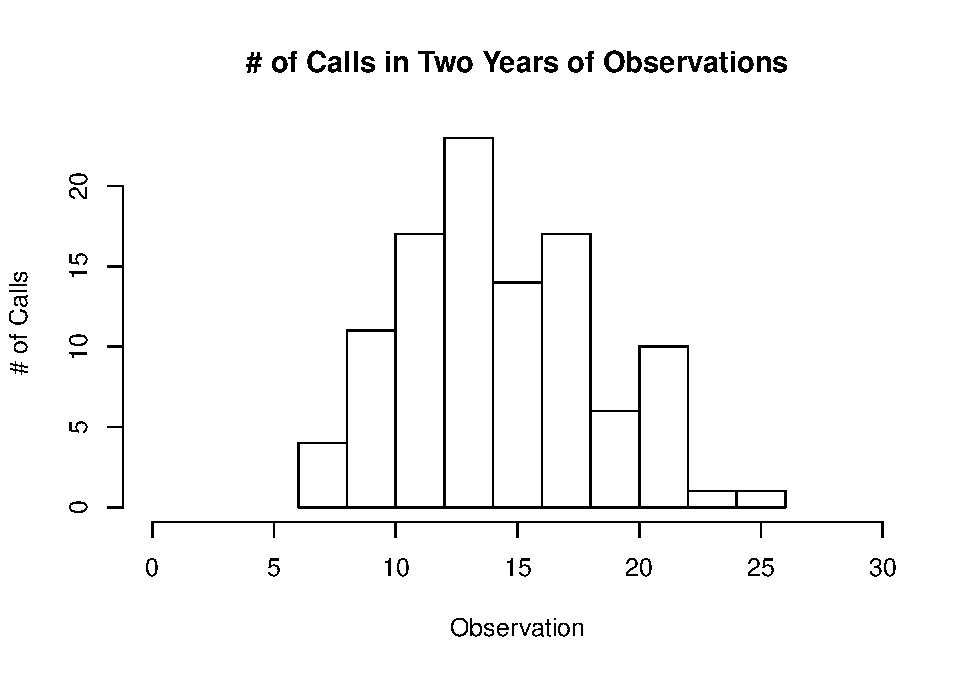
\includegraphics{Locker-Angelina-ADA-Homework-02_files/figure-latex/unnamed-chunk-7-1.pdf}

\begin{enumerate}
\def\labelenumi{\arabic{enumi}.}
\setcounter{enumi}{1}
\tightlist
\item
  Load in the dataset ``zombies.csv'' from my GitHub repository at
  \url{https://github.com/difiore/ADA-2019}. This data includes the
  first and last name and gender of the entire population of 1000 people
  who have survived the zombie apocalypse and are now ekeing out an
  existence somewhere on the East Coast, along with several other
  variables (height, weight, age, number of years of education, number
  of zombies they have killed, and college major see here for info on
  important post-zombie apocalypse majors
\end{enumerate}

\begin{Shaded}
\begin{Highlighting}[]
\NormalTok{d <-}\StringTok{ }\KeywordTok{read.csv}\NormalTok{(}\DataTypeTok{file =} \StringTok{"C:/Users/ajlocker/Desktop/Data Analysis/zombies.csv"}\NormalTok{, }\DataTypeTok{sep =} \StringTok{","}\NormalTok{, }\DataTypeTok{header =}  \OtherTok{TRUE}\NormalTok{, }\DataTypeTok{stringsAsFactors =} \OtherTok{FALSE}\NormalTok{)}
\KeywordTok{head}\NormalTok{(d)}
\end{Highlighting}
\end{Shaded}

\begin{verbatim}
##   id first_name last_name gender   height   weight zombies_killed
## 1  1      Sarah    Little Female 62.88951 132.0872              2
## 2  2       Mark    Duncan   Male 67.80277 146.3753              5
## 3  3    Brandon     Perez   Male 72.12908 152.9370              1
## 4  4      Roger   Coleman   Male 66.78484 129.7418              5
## 5  5      Tammy    Powell Female 64.71832 132.4265              4
## 6  6    Anthony     Green   Male 71.24326 152.5246              1
##   years_of_education                           major      age
## 1                  1                medicine/nursing 17.64275
## 2                  3 criminal justice administration 22.58951
## 3                  1                       education 21.91276
## 4                  6                  energy studies 18.19058
## 5                  3                       logistics 21.10399
## 6                  4                  energy studies 21.48355
\end{verbatim}

2.a. Calculate the population mean and standard deviation for each
quantitative random variable (height, weight, age, number of zombies
killed, and years of education). NOTE: You will not want to use the
built in var() and sd() commands as those are for samples.

\begin{Shaded}
\begin{Highlighting}[]
\KeywordTok{library}\NormalTok{(tidyverse)}
\end{Highlighting}
\end{Shaded}

\begin{verbatim}
## -- Attaching packages ------------------------------------------------------------------------------ tidyverse 1.2.1 --
\end{verbatim}

\begin{verbatim}
## v ggplot2 3.1.0     v purrr   0.3.0
## v tibble  2.0.1     v dplyr   0.7.8
## v tidyr   0.8.2     v stringr 1.3.1
## v readr   1.3.1     v forcats 0.3.0
\end{verbatim}

\begin{verbatim}
## -- Conflicts --------------------------------------------------------------------------------- tidyverse_conflicts() --
## x dplyr::filter() masks stats::filter()
## x dplyr::lag()    masks stats::lag()
\end{verbatim}

\begin{Shaded}
\begin{Highlighting}[]
\KeywordTok{library}\NormalTok{(psych)}
\end{Highlighting}
\end{Shaded}

\begin{verbatim}
## 
## Attaching package: 'psych'
\end{verbatim}

\begin{verbatim}
## The following objects are masked from 'package:ggplot2':
## 
##     %+%, alpha
\end{verbatim}

\begin{Shaded}
\begin{Highlighting}[]
\NormalTok{sel_data <-}\StringTok{ }\KeywordTok{select}\NormalTok{(d,height, age, weight, zombies_killed, years_of_education)}

\KeywordTok{describe}\NormalTok{(sel_data)}
\end{Highlighting}
\end{Shaded}

\begin{verbatim}
##                    vars    n   mean    sd median trimmed   mad   min
## height                1 1000  67.63  4.31  67.50   67.58  4.23 54.15
## age                   2 1000  20.05  2.97  19.90   20.01  2.88 10.66
## weight                3 1000 143.91 18.40 142.89  143.71 18.08 90.29
## zombies_killed        4 1000   2.99  1.75   3.00    2.87  1.48  0.00
## years_of_education    5 1000   3.00  1.68   3.00    2.92  1.48  0.00
##                       max  range skew kurtosis   se
## height              80.53  26.38 0.08    -0.01 0.14
## age                 29.59  18.93 0.13     0.10 0.09
## weight             210.79 120.50 0.13    -0.01 0.58
## zombies_killed      11.00  11.00 0.67     0.54 0.06
## years_of_education   8.00   8.00 0.40    -0.21 0.05
\end{verbatim}

\begin{Shaded}
\begin{Highlighting}[]
\NormalTok{sd_height <-}\StringTok{ }\KeywordTok{sqrt}\NormalTok{(}\KeywordTok{sum}\NormalTok{((d}\OperatorTok{$}\NormalTok{height}\OperatorTok{-}\KeywordTok{mean}\NormalTok{(d}\OperatorTok{$}\NormalTok{height))}\OperatorTok{^}\DecValTok{2}\NormalTok{)}\OperatorTok{/}\KeywordTok{length}\NormalTok{(d}\OperatorTok{$}\NormalTok{height))}
                                                   
\NormalTok{sd_weight <-}\StringTok{ }\KeywordTok{sqrt}\NormalTok{(}\KeywordTok{sum}\NormalTok{((d}\OperatorTok{$}\NormalTok{weight}\OperatorTok{-}\KeywordTok{mean}\NormalTok{(d}\OperatorTok{$}\NormalTok{weight))}\OperatorTok{^}\DecValTok{2}\NormalTok{)}\OperatorTok{/}\KeywordTok{length}\NormalTok{(d}\OperatorTok{$}\NormalTok{weight))}

\NormalTok{sd_age <-}\StringTok{ }\KeywordTok{sqrt}\NormalTok{(}\KeywordTok{sum}\NormalTok{((d}\OperatorTok{$}\NormalTok{age}\OperatorTok{-}\KeywordTok{mean}\NormalTok{(d}\OperatorTok{$}\NormalTok{age))}\OperatorTok{^}\DecValTok{2}\NormalTok{)}\OperatorTok{/}\KeywordTok{length}\NormalTok{(d}\OperatorTok{$}\NormalTok{age))}

\NormalTok{sd_kills <-}\StringTok{ }\KeywordTok{sqrt}\NormalTok{(}\KeywordTok{sum}\NormalTok{((d}\OperatorTok{$}\NormalTok{zombies_killed}\OperatorTok{-}\KeywordTok{mean}\NormalTok{(d}\OperatorTok{$}\NormalTok{zombies_killed))}\OperatorTok{^}\DecValTok{2}\NormalTok{)}\OperatorTok{/}\KeywordTok{length}\NormalTok{(d}\OperatorTok{$}\NormalTok{zombies_killed)) }

\NormalTok{sd_edu <-}\StringTok{ }\KeywordTok{sqrt}\NormalTok{(}\KeywordTok{sum}\NormalTok{((d}\OperatorTok{$}\NormalTok{years_of_education}\OperatorTok{-}\KeywordTok{mean}\NormalTok{(d}\OperatorTok{$}\NormalTok{years_of_education))}\OperatorTok{^}\DecValTok{2}\NormalTok{)}\OperatorTok{/}\KeywordTok{length}\NormalTok{(d}\OperatorTok{$}\NormalTok{years_of_education)) }

\NormalTok{mean_height <-}\StringTok{ }\KeywordTok{mean}\NormalTok{(d}\OperatorTok{$}\NormalTok{height)}

\NormalTok{mean_weight <-}\StringTok{ }\KeywordTok{mean}\NormalTok{(d}\OperatorTok{$}\NormalTok{weight)}

\NormalTok{mean_age <-}\StringTok{ }\KeywordTok{mean}\NormalTok{(d}\OperatorTok{$}\NormalTok{age)}

\NormalTok{mean_kills <-}\StringTok{ }\KeywordTok{mean}\NormalTok{(d}\OperatorTok{$}\NormalTok{zombies_killed)}

\NormalTok{mean_edu <-}\StringTok{ }\KeywordTok{mean}\NormalTok{(d}\OperatorTok{$}\NormalTok{years_of_education)}


\NormalTok{sd_height}
\end{Highlighting}
\end{Shaded}

\begin{verbatim}
## [1] 4.30797
\end{verbatim}

\begin{Shaded}
\begin{Highlighting}[]
\NormalTok{sd_age}
\end{Highlighting}
\end{Shaded}

\begin{verbatim}
## [1] 2.963583
\end{verbatim}

\begin{Shaded}
\begin{Highlighting}[]
\NormalTok{sd_weight}
\end{Highlighting}
\end{Shaded}

\begin{verbatim}
## [1] 18.39186
\end{verbatim}

\begin{Shaded}
\begin{Highlighting}[]
\NormalTok{sd_kills}
\end{Highlighting}
\end{Shaded}

\begin{verbatim}
## [1] 1.747551
\end{verbatim}

\begin{Shaded}
\begin{Highlighting}[]
\NormalTok{sd_edu}
\end{Highlighting}
\end{Shaded}

\begin{verbatim}
## [1] 1.675704
\end{verbatim}

\begin{Shaded}
\begin{Highlighting}[]
\NormalTok{mean_height}
\end{Highlighting}
\end{Shaded}

\begin{verbatim}
## [1] 67.6301
\end{verbatim}

\begin{Shaded}
\begin{Highlighting}[]
\NormalTok{mean_age}
\end{Highlighting}
\end{Shaded}

\begin{verbatim}
## [1] 20.04696
\end{verbatim}

\begin{Shaded}
\begin{Highlighting}[]
\NormalTok{mean_weight}
\end{Highlighting}
\end{Shaded}

\begin{verbatim}
## [1] 143.9075
\end{verbatim}

\begin{Shaded}
\begin{Highlighting}[]
\NormalTok{mean_kills}
\end{Highlighting}
\end{Shaded}

\begin{verbatim}
## [1] 2.992
\end{verbatim}

\begin{Shaded}
\begin{Highlighting}[]
\NormalTok{mean_edu}
\end{Highlighting}
\end{Shaded}

\begin{verbatim}
## [1] 2.996
\end{verbatim}

2.b. Use \{ggplot\} and make boxplots of each of these variable by
gender.

\begin{Shaded}
\begin{Highlighting}[]
\KeywordTok{library}\NormalTok{(tidyverse)}
\KeywordTok{library}\NormalTok{(ggplot2)}
\NormalTok{abox <-}\StringTok{ }\KeywordTok{ggplot}\NormalTok{(}\DataTypeTok{data =}\NormalTok{ d, }\KeywordTok{aes}\NormalTok{(}\DataTypeTok{x =}\NormalTok{ gender, }\DataTypeTok{y =}\NormalTok{ age, }\DataTypeTok{color =}\NormalTok{ gender)) }\OperatorTok{+}\StringTok{ }\KeywordTok{xlab}\NormalTok{(}\StringTok{"Gender"}\NormalTok{) }\OperatorTok{+}\StringTok{ }\KeywordTok{ylab}\NormalTok{(}\StringTok{"Age"}\NormalTok{) }\OperatorTok{+}\StringTok{ }\KeywordTok{geom_boxplot}\NormalTok{(}\DataTypeTok{na.rm =} \OtherTok{TRUE}\NormalTok{) }\OperatorTok{+}\StringTok{ }\KeywordTok{theme}\NormalTok{(}\DataTypeTok{legend.position =} \StringTok{"bottom"}\NormalTok{, }\DataTypeTok{legend.title =} \KeywordTok{element_blank}\NormalTok{())}
\NormalTok{abox}
\end{Highlighting}
\end{Shaded}

\includegraphics{Locker-Angelina-ADA-Homework-02_files/figure-latex/unnamed-chunk-10-1.pdf}

\begin{Shaded}
\begin{Highlighting}[]
\NormalTok{wbox <-}\StringTok{ }\KeywordTok{ggplot}\NormalTok{(}\DataTypeTok{data =}\NormalTok{ d, }\KeywordTok{aes}\NormalTok{(}\DataTypeTok{x =}\NormalTok{ gender, }\DataTypeTok{y =}\NormalTok{ weight, }\DataTypeTok{color =}\NormalTok{ gender)) }\OperatorTok{+}\StringTok{ }\KeywordTok{xlab}\NormalTok{(}\StringTok{"Gender"}\NormalTok{) }\OperatorTok{+}\StringTok{ }\KeywordTok{ylab}\NormalTok{(}\StringTok{"Weight"}\NormalTok{) }\OperatorTok{+}\StringTok{ }\KeywordTok{geom_boxplot}\NormalTok{(}\DataTypeTok{na.rm =} \OtherTok{TRUE}\NormalTok{) }\OperatorTok{+}\StringTok{ }\KeywordTok{theme}\NormalTok{(}\DataTypeTok{legend.position =} \StringTok{"bottom"}\NormalTok{, }\DataTypeTok{legend.title =} \KeywordTok{element_blank}\NormalTok{())}
\NormalTok{wbox}
\end{Highlighting}
\end{Shaded}

\includegraphics{Locker-Angelina-ADA-Homework-02_files/figure-latex/unnamed-chunk-10-2.pdf}

\begin{Shaded}
\begin{Highlighting}[]
\NormalTok{hbox <-}\StringTok{ }\KeywordTok{ggplot}\NormalTok{(}\DataTypeTok{data =}\NormalTok{ d, }\KeywordTok{aes}\NormalTok{(}\DataTypeTok{x =}\NormalTok{ gender, }\DataTypeTok{y =}\NormalTok{ height, }\DataTypeTok{color =}\NormalTok{ gender)) }\OperatorTok{+}\StringTok{ }\KeywordTok{xlab}\NormalTok{(}\StringTok{"Gender"}\NormalTok{) }\OperatorTok{+}\StringTok{ }\KeywordTok{ylab}\NormalTok{(}\StringTok{"Height"}\NormalTok{) }\OperatorTok{+}\StringTok{ }\KeywordTok{geom_boxplot}\NormalTok{(}\DataTypeTok{na.rm =} \OtherTok{TRUE}\NormalTok{) }\OperatorTok{+}\StringTok{ }\KeywordTok{theme}\NormalTok{(}\DataTypeTok{legend.position =} \StringTok{"bottom"}\NormalTok{, }\DataTypeTok{legend.title =} \KeywordTok{element_blank}\NormalTok{())}
\NormalTok{hbox}
\end{Highlighting}
\end{Shaded}

\includegraphics{Locker-Angelina-ADA-Homework-02_files/figure-latex/unnamed-chunk-10-3.pdf}

\begin{Shaded}
\begin{Highlighting}[]
\NormalTok{zbox <-}\StringTok{ }\KeywordTok{ggplot}\NormalTok{(}\DataTypeTok{data =}\NormalTok{ d, }\KeywordTok{aes}\NormalTok{(}\DataTypeTok{x =}\NormalTok{ gender, }\DataTypeTok{y =}\NormalTok{ zombies_killed, }\DataTypeTok{color =}\NormalTok{ gender)) }\OperatorTok{+}\StringTok{ }\KeywordTok{xlab}\NormalTok{(}\StringTok{"Gender"}\NormalTok{) }\OperatorTok{+}\StringTok{ }\KeywordTok{ylab}\NormalTok{(}\StringTok{"Kills"}\NormalTok{) }\OperatorTok{+}\StringTok{ }\KeywordTok{geom_boxplot}\NormalTok{(}\DataTypeTok{na.rm =} \OtherTok{TRUE}\NormalTok{) }\OperatorTok{+}\StringTok{ }\KeywordTok{theme}\NormalTok{(}\DataTypeTok{legend.position =} \StringTok{"bottom"}\NormalTok{, }\DataTypeTok{legend.title =} \KeywordTok{element_blank}\NormalTok{())}
\NormalTok{zbox}
\end{Highlighting}
\end{Shaded}

\includegraphics{Locker-Angelina-ADA-Homework-02_files/figure-latex/unnamed-chunk-10-4.pdf}

\begin{Shaded}
\begin{Highlighting}[]
\NormalTok{ebox <-}\StringTok{ }\KeywordTok{ggplot}\NormalTok{(}\DataTypeTok{data =}\NormalTok{ d, }\KeywordTok{aes}\NormalTok{(}\DataTypeTok{x =}\NormalTok{ gender, }\DataTypeTok{y =}\NormalTok{ years_of_education, }\DataTypeTok{color =}\NormalTok{ gender)) }\OperatorTok{+}\StringTok{ }\KeywordTok{xlab}\NormalTok{(}\StringTok{"Gender"}\NormalTok{) }\OperatorTok{+}\StringTok{ }\KeywordTok{ylab}\NormalTok{(}\StringTok{"Education"}\NormalTok{) }\OperatorTok{+}\StringTok{ }\KeywordTok{geom_boxplot}\NormalTok{(}\DataTypeTok{na.rm =} \OtherTok{TRUE}\NormalTok{) }\OperatorTok{+}\StringTok{ }\KeywordTok{theme}\NormalTok{(}\DataTypeTok{legend.position =} \StringTok{"bottom"}\NormalTok{, }\DataTypeTok{legend.title =} \KeywordTok{element_blank}\NormalTok{())}
\NormalTok{ebox}
\end{Highlighting}
\end{Shaded}

\includegraphics{Locker-Angelina-ADA-Homework-02_files/figure-latex/unnamed-chunk-10-5.pdf}

2.c. Use \{ggplot\} and make scatterplots of height and weight in
relation to age. Do these variables seem to be related? In what way?
\emph{Both height and weight, in relation to age, have positive linear
correlations. Height and age is a stong(ish) positive linear
correlation; weight and age is a weak positive linear correlation}

\begin{Shaded}
\begin{Highlighting}[]
\NormalTok{hscat <-}\StringTok{ }\KeywordTok{ggplot}\NormalTok{(}\DataTypeTok{data =}\NormalTok{ d, }\KeywordTok{aes}\NormalTok{(}\DataTypeTok{x =}\NormalTok{ age, }\DataTypeTok{y =}\NormalTok{ height)) }\OperatorTok{+}\StringTok{ }\KeywordTok{xlab}\NormalTok{(}\StringTok{"Age"}\NormalTok{) }\OperatorTok{+}\StringTok{ }\KeywordTok{ylab}\NormalTok{(}\StringTok{"Height"}\NormalTok{) }\OperatorTok{+}\StringTok{ }\KeywordTok{geom_point}\NormalTok{(}\DataTypeTok{na.rm =} \OtherTok{TRUE}\NormalTok{) }\OperatorTok{+}\StringTok{ }\KeywordTok{theme}\NormalTok{(}\DataTypeTok{legend.position =} \StringTok{"bottom"}\NormalTok{, }\DataTypeTok{legend.title =} \KeywordTok{element_blank}\NormalTok{())}
\NormalTok{hscat}
\end{Highlighting}
\end{Shaded}

\includegraphics{Locker-Angelina-ADA-Homework-02_files/figure-latex/unnamed-chunk-11-1.pdf}

\begin{Shaded}
\begin{Highlighting}[]
\NormalTok{wscat <-}\StringTok{ }\KeywordTok{ggplot}\NormalTok{(}\DataTypeTok{data =}\NormalTok{ d, }\KeywordTok{aes}\NormalTok{(}\DataTypeTok{x =}\NormalTok{ age, }\DataTypeTok{y =}\NormalTok{ weight)) }\OperatorTok{+}\StringTok{ }\KeywordTok{xlab}\NormalTok{(}\StringTok{"Age"}\NormalTok{) }\OperatorTok{+}\StringTok{ }\KeywordTok{ylab}\NormalTok{(}\StringTok{"Weight"}\NormalTok{) }\OperatorTok{+}\StringTok{ }\KeywordTok{geom_point}\NormalTok{(}\DataTypeTok{na.rm =} \OtherTok{TRUE}\NormalTok{) }\OperatorTok{+}\StringTok{ }\KeywordTok{theme}\NormalTok{(}\DataTypeTok{legend.position =} \StringTok{"bottom"}\NormalTok{, }\DataTypeTok{legend.title =} \KeywordTok{element_blank}\NormalTok{())}
\NormalTok{wscat}
\end{Highlighting}
\end{Shaded}

\includegraphics{Locker-Angelina-ADA-Homework-02_files/figure-latex/unnamed-chunk-11-2.pdf}

2.d. Using histograms and Q-Q plots, check whether the quantitative
variables seem to be drawn from a normal distribution. Which seem to be
and which do not? \emph{Kills and Edu are not from normal distributions}

\begin{Shaded}
\begin{Highlighting}[]
\KeywordTok{hist}\NormalTok{(d}\OperatorTok{$}\NormalTok{age)}
\end{Highlighting}
\end{Shaded}

\includegraphics{Locker-Angelina-ADA-Homework-02_files/figure-latex/unnamed-chunk-12-1.pdf}

\begin{Shaded}
\begin{Highlighting}[]
\KeywordTok{hist}\NormalTok{(d}\OperatorTok{$}\NormalTok{weight)}
\end{Highlighting}
\end{Shaded}

\includegraphics{Locker-Angelina-ADA-Homework-02_files/figure-latex/unnamed-chunk-12-2.pdf}

\begin{Shaded}
\begin{Highlighting}[]
\KeywordTok{hist}\NormalTok{(d}\OperatorTok{$}\NormalTok{height)}
\end{Highlighting}
\end{Shaded}

\includegraphics{Locker-Angelina-ADA-Homework-02_files/figure-latex/unnamed-chunk-12-3.pdf}

\begin{Shaded}
\begin{Highlighting}[]
\KeywordTok{hist}\NormalTok{(d}\OperatorTok{$}\NormalTok{zombies_killed)}
\end{Highlighting}
\end{Shaded}

\includegraphics{Locker-Angelina-ADA-Homework-02_files/figure-latex/unnamed-chunk-12-4.pdf}

\begin{Shaded}
\begin{Highlighting}[]
\KeywordTok{hist}\NormalTok{(d}\OperatorTok{$}\NormalTok{years_of_education)}
\end{Highlighting}
\end{Shaded}

\includegraphics{Locker-Angelina-ADA-Homework-02_files/figure-latex/unnamed-chunk-12-5.pdf}

\begin{Shaded}
\begin{Highlighting}[]
\KeywordTok{qqnorm}\NormalTok{(d}\OperatorTok{$}\NormalTok{age, }\DataTypeTok{main =} \StringTok{"QQ Age"}\NormalTok{)}
\KeywordTok{qqline}\NormalTok{(d}\OperatorTok{$}\NormalTok{age, }\DataTypeTok{col =} \StringTok{"gray"}\NormalTok{)}
\end{Highlighting}
\end{Shaded}

\includegraphics{Locker-Angelina-ADA-Homework-02_files/figure-latex/unnamed-chunk-12-6.pdf}

\begin{Shaded}
\begin{Highlighting}[]
\KeywordTok{qqnorm}\NormalTok{(d}\OperatorTok{$}\NormalTok{weight, }\DataTypeTok{main =} \StringTok{"QQ Weight"}\NormalTok{)}
\KeywordTok{qqline}\NormalTok{(d}\OperatorTok{$}\NormalTok{weight, }\DataTypeTok{col =} \StringTok{"gray"}\NormalTok{)}
\end{Highlighting}
\end{Shaded}

\includegraphics{Locker-Angelina-ADA-Homework-02_files/figure-latex/unnamed-chunk-12-7.pdf}

\begin{Shaded}
\begin{Highlighting}[]
\KeywordTok{qqnorm}\NormalTok{(d}\OperatorTok{$}\NormalTok{height, }\DataTypeTok{main =} \StringTok{"QQ Height"}\NormalTok{)}
\KeywordTok{qqline}\NormalTok{(d}\OperatorTok{$}\NormalTok{height, }\DataTypeTok{col =} \StringTok{"gray"}\NormalTok{)}
\end{Highlighting}
\end{Shaded}

\includegraphics{Locker-Angelina-ADA-Homework-02_files/figure-latex/unnamed-chunk-12-8.pdf}

\begin{Shaded}
\begin{Highlighting}[]
\KeywordTok{qqnorm}\NormalTok{(d}\OperatorTok{$}\NormalTok{zombies_killed, }\DataTypeTok{main =} \StringTok{"QQ Kills"}\NormalTok{)}
\KeywordTok{qqline}\NormalTok{(d}\OperatorTok{$}\NormalTok{zombies_killed, }\DataTypeTok{col =} \StringTok{"gray"}\NormalTok{)}
\end{Highlighting}
\end{Shaded}

\includegraphics{Locker-Angelina-ADA-Homework-02_files/figure-latex/unnamed-chunk-12-9.pdf}

\begin{Shaded}
\begin{Highlighting}[]
\KeywordTok{qqnorm}\NormalTok{(d}\OperatorTok{$}\NormalTok{years_of_education, }\DataTypeTok{main =} \StringTok{"QQ Education"}\NormalTok{)}
\KeywordTok{qqline}\NormalTok{(d}\OperatorTok{$}\NormalTok{years_of_education, }\DataTypeTok{col =} \StringTok{"gray"}\NormalTok{)}
\end{Highlighting}
\end{Shaded}

\includegraphics{Locker-Angelina-ADA-Homework-02_files/figure-latex/unnamed-chunk-12-10.pdf}

HINT: Not all are drawn from a normal distribution! For those that are
not, can you determine what common distribution they are drawn from?

2.e. Now use the sample() function to sample ONE subset of 30 zombies
(without replacement) from this population and calculate the mean and
sample standard deviation for each variable. Also estimate the standard
error for each variable and construct the 95\% confidence interval for
each mean. Note that for the variables that are not drawn from the
normal distribution, you will need to base your estimate of the CIs on
some different distribution!

\begin{Shaded}
\begin{Highlighting}[]
\NormalTok{k <-}\StringTok{ }\DecValTok{1}  \CommentTok{# number of subsets taken}
\NormalTok{n <-}\StringTok{ }\DecValTok{30}  \CommentTok{# subset size}
\NormalTok{group <-}\StringTok{ }\OtherTok{NULL}  \CommentTok{# dummy}

\ControlFlowTok{for}\NormalTok{ (i }\ControlFlowTok{in} \DecValTok{1}\OperatorTok{:}\NormalTok{k) \{}
\NormalTok{  group <-}\StringTok{ }\KeywordTok{sample}\NormalTok{(}\DecValTok{1}\OperatorTok{:}\KeywordTok{nrow}\NormalTok{(sel_data), }\DataTypeTok{size =}\NormalTok{ n, }\DataTypeTok{replace =} \OtherTok{FALSE}\NormalTok{)}
\NormalTok{\}}

\NormalTok{x <-}\StringTok{ }\NormalTok{sel_data[group, ]}
\NormalTok{x}
\end{Highlighting}
\end{Shaded}

\begin{verbatim}
##       height      age   weight zombies_killed years_of_education
## 463 74.83504 21.22975 157.0047              2                  4
## 924 72.60485 22.86708 185.7961              5                  3
## 333 67.47215 20.61760 126.4773              6                  2
## 32  70.99726 20.34347 158.8277              1                  0
## 335 68.16540 20.03842 152.7236              1                  2
## 787 66.35376 23.80758 131.4980              2                  3
## 192 64.81685 16.95885 136.7623              4                  0
## 52  60.66651 21.27616 103.6431              2                  0
## 508 60.56442 16.50589 116.3655              4                  5
## 59  69.04027 21.72433 159.6951              6                  6
## 241 65.73552 23.26286 131.2713              2                  3
## 958 62.06469 17.19527 137.5064              3                  1
## 597 63.14829 21.91993 106.4643              2                  0
## 24  68.40552 21.69196 151.4956              3                  3
## 705 68.02251 19.02552 171.4614              3                  6
## 234 69.19429 22.91233 149.2429              6                  2
## 284 58.13216 16.98641 110.8869              3                  4
## 882 63.84095 17.01380 137.0027              2                  4
## 625 64.62151 17.31604 120.7034              9                  2
## 425 67.17895 20.28953 145.1002              5                  0
## 27  64.27576 21.07451 122.7359              1                  2
## 984 61.04618 19.27299 105.6838              1                  0
## 30  69.14401 23.76366 149.1776              1                  1
## 169 70.31931 27.40790 143.8071              2                  4
## 753 68.03470 19.89604 143.6416              2                  3
## 540 62.43483 18.06575 112.0983              3                  2
## 397 61.58678 16.19753 132.1894              0                  5
## 468 70.73679 18.45236 152.0145              3                  4
## 650 66.52055 16.85585 135.8782              3                  3
## 356 70.42895 23.05967 134.4735              2                  4
\end{verbatim}

** means**

\begin{Shaded}
\begin{Highlighting}[]
\NormalTok{hm <-}\StringTok{ }\KeywordTok{mean}\NormalTok{(x}\OperatorTok{$}\NormalTok{height)}
\NormalTok{hm}
\end{Highlighting}
\end{Shaded}

\begin{verbatim}
## [1] 66.34629
\end{verbatim}

\begin{Shaded}
\begin{Highlighting}[]
\NormalTok{am <-}\StringTok{ }\KeywordTok{mean}\NormalTok{(x}\OperatorTok{$}\NormalTok{age)}
\NormalTok{am}
\end{Highlighting}
\end{Shaded}

\begin{verbatim}
## [1] 20.2343
\end{verbatim}

\begin{Shaded}
\begin{Highlighting}[]
\NormalTok{wm <-}\StringTok{ }\KeywordTok{mean}\NormalTok{(x}\OperatorTok{$}\NormalTok{weight)}
\NormalTok{wm}
\end{Highlighting}
\end{Shaded}

\begin{verbatim}
## [1] 137.3876
\end{verbatim}

\begin{Shaded}
\begin{Highlighting}[]
\NormalTok{zm <-}\StringTok{ }\KeywordTok{mean}\NormalTok{(x}\OperatorTok{$}\NormalTok{zombies_killed)}
\NormalTok{zm}
\end{Highlighting}
\end{Shaded}

\begin{verbatim}
## [1] 2.966667
\end{verbatim}

\begin{Shaded}
\begin{Highlighting}[]
\NormalTok{em <-}\StringTok{ }\KeywordTok{mean}\NormalTok{(x}\OperatorTok{$}\NormalTok{years_of_education)}
\NormalTok{em}
\end{Highlighting}
\end{Shaded}

\begin{verbatim}
## [1] 2.6
\end{verbatim}

** standard deviations**

\begin{Shaded}
\begin{Highlighting}[]
\NormalTok{hsd <-}\StringTok{ }\KeywordTok{sd}\NormalTok{(x}\OperatorTok{$}\NormalTok{height)}
\NormalTok{hsd}
\end{Highlighting}
\end{Shaded}

\begin{verbatim}
## [1] 4.012921
\end{verbatim}

\begin{Shaded}
\begin{Highlighting}[]
\NormalTok{asd <-}\StringTok{ }\KeywordTok{sd}\NormalTok{(x}\OperatorTok{$}\NormalTok{age)}
\NormalTok{asd}
\end{Highlighting}
\end{Shaded}

\begin{verbatim}
## [1] 2.751183
\end{verbatim}

\begin{Shaded}
\begin{Highlighting}[]
\NormalTok{wsd <-}\StringTok{ }\KeywordTok{sd}\NormalTok{(x}\OperatorTok{$}\NormalTok{weight)}
\NormalTok{wsd}
\end{Highlighting}
\end{Shaded}

\begin{verbatim}
## [1] 19.93129
\end{verbatim}

\begin{Shaded}
\begin{Highlighting}[]
\NormalTok{zsd <-}\StringTok{ }\KeywordTok{sd}\NormalTok{(x}\OperatorTok{$}\NormalTok{zombies_killed)}
\NormalTok{zsd}
\end{Highlighting}
\end{Shaded}

\begin{verbatim}
## [1] 1.956128
\end{verbatim}

\begin{Shaded}
\begin{Highlighting}[]
\NormalTok{esd <-}\StringTok{ }\KeywordTok{sd}\NormalTok{(x}\OperatorTok{$}\NormalTok{years_of_education)}
\NormalTok{esd}
\end{Highlighting}
\end{Shaded}

\begin{verbatim}
## [1] 1.811838
\end{verbatim}

\textbf{standard errors}

\begin{Shaded}
\begin{Highlighting}[]
\KeywordTok{library}\NormalTok{(sciplot)}
\NormalTok{hse <-}\StringTok{ }\KeywordTok{se}\NormalTok{(x}\OperatorTok{$}\NormalTok{height)}
\NormalTok{hse}
\end{Highlighting}
\end{Shaded}

\begin{verbatim}
## [1] 0.7326557
\end{verbatim}

\begin{Shaded}
\begin{Highlighting}[]
\NormalTok{ase <-}\StringTok{ }\KeywordTok{se}\NormalTok{(x}\OperatorTok{$}\NormalTok{age)}
\NormalTok{ase}
\end{Highlighting}
\end{Shaded}

\begin{verbatim}
## [1] 0.5022951
\end{verbatim}

\begin{Shaded}
\begin{Highlighting}[]
\NormalTok{wse <-}\StringTok{ }\KeywordTok{se}\NormalTok{(x}\OperatorTok{$}\NormalTok{weight)}
\NormalTok{wse}
\end{Highlighting}
\end{Shaded}

\begin{verbatim}
## [1] 3.638938
\end{verbatim}

\begin{Shaded}
\begin{Highlighting}[]
\NormalTok{zse <-}\StringTok{ }\KeywordTok{se}\NormalTok{(x}\OperatorTok{$}\NormalTok{zombies_killed)}
\NormalTok{zse}
\end{Highlighting}
\end{Shaded}

\begin{verbatim}
## [1] 0.3571385
\end{verbatim}

\begin{Shaded}
\begin{Highlighting}[]
\NormalTok{ese <-}\StringTok{ }\KeywordTok{se}\NormalTok{(x}\OperatorTok{$}\NormalTok{years_of_education)}
\NormalTok{ese}
\end{Highlighting}
\end{Shaded}

\begin{verbatim}
## [1] 0.3307949
\end{verbatim}

\textbf{confidence intervals}

\begin{Shaded}
\begin{Highlighting}[]
\NormalTok{upperheight <-}\StringTok{ }\NormalTok{hm }\OperatorTok{+}\StringTok{ }\KeywordTok{qnorm}\NormalTok{(}\FloatTok{0.975}\NormalTok{, }\DataTypeTok{mean =} \DecValTok{0}\NormalTok{, }\DataTypeTok{sd =} \DecValTok{1}\NormalTok{) }\OperatorTok{*}\StringTok{ }\NormalTok{hse}
\NormalTok{lowerheight <-}\StringTok{ }\NormalTok{hm }\OperatorTok{+}\StringTok{ }\KeywordTok{qnorm}\NormalTok{(}\FloatTok{0.025}\NormalTok{, }\DataTypeTok{mean =} \DecValTok{0}\NormalTok{, }\DataTypeTok{sd =} \DecValTok{1}\NormalTok{) }\OperatorTok{*}\StringTok{ }\NormalTok{hse }
\NormalTok{hci <-}\StringTok{ }\KeywordTok{c}\NormalTok{(lowerheight, upperheight)}
\NormalTok{hci}
\end{Highlighting}
\end{Shaded}

\begin{verbatim}
## [1] 64.91031 67.78227
\end{verbatim}

\begin{Shaded}
\begin{Highlighting}[]
\NormalTok{upperage <-}\StringTok{ }\NormalTok{am }\OperatorTok{+}\StringTok{ }\KeywordTok{qnorm}\NormalTok{(}\FloatTok{0.975}\NormalTok{, }\DataTypeTok{mean =} \DecValTok{0}\NormalTok{, }\DataTypeTok{sd =} \DecValTok{1}\NormalTok{) }\OperatorTok{*}\StringTok{ }\NormalTok{ase}
\NormalTok{lowerage <-}\StringTok{ }\NormalTok{am }\OperatorTok{+}\StringTok{ }\KeywordTok{qnorm}\NormalTok{(}\FloatTok{0.025}\NormalTok{, }\DataTypeTok{mean =} \DecValTok{0}\NormalTok{, }\DataTypeTok{sd =} \DecValTok{1}\NormalTok{) }\OperatorTok{*}\StringTok{ }\NormalTok{ase }
\NormalTok{aci <-}\StringTok{ }\KeywordTok{c}\NormalTok{(lowerage, upperage)}
\NormalTok{aci}
\end{Highlighting}
\end{Shaded}

\begin{verbatim}
## [1] 19.24982 21.21878
\end{verbatim}

\begin{Shaded}
\begin{Highlighting}[]
\NormalTok{upperweight <-}\StringTok{ }\NormalTok{wm }\OperatorTok{+}\StringTok{ }\KeywordTok{qnorm}\NormalTok{(}\FloatTok{0.975}\NormalTok{, }\DataTypeTok{mean =} \DecValTok{0}\NormalTok{, }\DataTypeTok{sd =} \DecValTok{1}\NormalTok{) }\OperatorTok{*}\StringTok{ }\NormalTok{wse}
\NormalTok{lowerweight <-}\StringTok{ }\NormalTok{wm }\OperatorTok{+}\StringTok{ }\KeywordTok{qnorm}\NormalTok{(}\FloatTok{0.025}\NormalTok{, }\DataTypeTok{mean =} \DecValTok{0}\NormalTok{, }\DataTypeTok{sd =} \DecValTok{1}\NormalTok{) }\OperatorTok{*}\StringTok{ }\NormalTok{wse }
\NormalTok{wci <-}\StringTok{ }\KeywordTok{c}\NormalTok{(lowerweight, upperweight)}
\NormalTok{wci}
\end{Highlighting}
\end{Shaded}

\begin{verbatim}
## [1] 130.2554 144.5198
\end{verbatim}

\begin{Shaded}
\begin{Highlighting}[]
\NormalTok{upperkills <-}\StringTok{ }\NormalTok{zm }\OperatorTok{+}\StringTok{ }\KeywordTok{qnorm}\NormalTok{(}\FloatTok{0.975}\NormalTok{, }\DataTypeTok{mean =} \DecValTok{0}\NormalTok{, }\DataTypeTok{sd =} \DecValTok{1}\NormalTok{) }\OperatorTok{*}\StringTok{ }\NormalTok{zse}
\NormalTok{lowerkills <-}\StringTok{ }\NormalTok{zm }\OperatorTok{+}\StringTok{ }\KeywordTok{qnorm}\NormalTok{(}\FloatTok{0.025}\NormalTok{, }\DataTypeTok{mean =} \DecValTok{0}\NormalTok{, }\DataTypeTok{sd =} \DecValTok{1}\NormalTok{) }\OperatorTok{*}\StringTok{ }\NormalTok{zse }
\NormalTok{zci <-}\StringTok{ }\KeywordTok{c}\NormalTok{(lowerkills, upperkills)}
\NormalTok{zci}
\end{Highlighting}
\end{Shaded}

\begin{verbatim}
## [1] 2.266688 3.666645
\end{verbatim}

\begin{Shaded}
\begin{Highlighting}[]
\NormalTok{upperedu <-}\StringTok{ }\NormalTok{em }\OperatorTok{+}\StringTok{ }\KeywordTok{qnorm}\NormalTok{(}\FloatTok{0.975}\NormalTok{, }\DataTypeTok{mean =} \DecValTok{0}\NormalTok{, }\DataTypeTok{sd =} \DecValTok{1}\NormalTok{) }\OperatorTok{*}\StringTok{ }\NormalTok{ese}
\NormalTok{loweredu <-}\StringTok{ }\NormalTok{em }\OperatorTok{+}\StringTok{ }\KeywordTok{qnorm}\NormalTok{(}\FloatTok{0.025}\NormalTok{, }\DataTypeTok{mean =} \DecValTok{0}\NormalTok{, }\DataTypeTok{sd =} \DecValTok{1}\NormalTok{) }\OperatorTok{*}\StringTok{ }\NormalTok{ese }
\NormalTok{eci <-}\StringTok{ }\KeywordTok{c}\NormalTok{(loweredu, upperedu)}
\NormalTok{eci}
\end{Highlighting}
\end{Shaded}

\begin{verbatim}
## [1] 1.951654 3.248346
\end{verbatim}

2.f. Now draw 99 more random samples of 30 zombies out and calculate the
mean for each of the these samples. Together with the first sample you
drew out, you now have a set of 100 means for each variable (each based
on 30 observations), which constitutes a sampling distribution for each
variable. What are the means and standard deviations of the sampling
distribution for each variable?

\begin{Shaded}
\begin{Highlighting}[]
\KeywordTok{set.seed}\NormalTok{(}\DecValTok{1}\NormalTok{)}
\NormalTok{k <-}\StringTok{ }\DecValTok{99}  \CommentTok{# number of subsets taken}
\NormalTok{n <-}\StringTok{ }\DecValTok{30}  \CommentTok{# subset size}
\NormalTok{biggroup <-}\StringTok{ }\OtherTok{NULL}  \CommentTok{# dummy}

\ControlFlowTok{for}\NormalTok{ (i }\ControlFlowTok{in} \DecValTok{1}\OperatorTok{:}\DecValTok{99}\NormalTok{) \{}
\NormalTok{  biggroup[[i]] <-}\StringTok{ }\KeywordTok{sample}\NormalTok{(}\DecValTok{1}\OperatorTok{:}\KeywordTok{nrow}\NormalTok{(sel_data), }\DataTypeTok{size =} \DecValTok{30}\NormalTok{, }\DataTypeTok{replace =} \OtherTok{FALSE}\NormalTok{)}
\NormalTok{\}}

\NormalTok{t <-}\StringTok{ }\NormalTok{sel_data[biggroup[[i]], ]}
\NormalTok{t}
\end{Highlighting}
\end{Shaded}

\begin{verbatim}
##       height      age   weight zombies_killed years_of_education
## 63  63.16399 16.78669 126.6091              1                  3
## 997 66.48566 19.87402 157.0878              3                  2
## 114 72.66829 19.19078 176.6687              2                  3
## 624 63.42365 17.07766 131.4085              2                  3
## 26  66.21361 18.82527 147.5891              1                  3
## 69  67.17319 20.81643 137.0979              1                  2
## 188 71.49300 19.91412 162.2126              5                  3
## 795 70.09081 16.55408 160.1624              5                  3
## 829 63.24188 18.85515 128.4248              1                  3
## 719 73.81399 27.37130 159.5498              4                  3
## 278 74.59113 20.23903 183.0497              7                  4
## 636 69.74712 20.39527 143.6522              1                  3
## 948 70.19100 23.41001 160.5423              2                  1
## 531 69.32048 24.53695 140.0381              2                  2
## 426 68.58895 21.32987 139.3016              3                  3
## 714 66.26057 17.36132 158.5050              3                  1
## 172 69.38269 25.74573 140.2724              4                  4
## 315 65.69532 20.38294 123.4174              5                  4
## 381 60.59620 15.60612 124.3349              2                  3
## 54  62.42483 18.29770 140.5250              1                  0
## 273 62.65719 18.50000 148.3196              2                  3
## 701 67.38798 19.64791 146.0300              1                  3
## 322 63.74886 18.75647 131.5360              3                  6
## 588 65.74474 19.78770 126.9184              2                  1
## 512 75.86921 23.43548 181.7209              4                  2
## 840 66.41866 21.11497 140.7097              4                  4
## 519 68.49669 16.22865 158.3162              0                  5
## 109 69.63299 24.14089 140.8563              5                  5
## 755 66.13981 22.98415 125.8349              4                  0
## 62  67.60233 19.97048 145.2308              3                  2
\end{verbatim}

\begin{Shaded}
\begin{Highlighting}[]
\NormalTok{y <-}\StringTok{ }\KeywordTok{rbind}\NormalTok{(t, x)}
\NormalTok{y}
\end{Highlighting}
\end{Shaded}

\begin{verbatim}
##       height      age   weight zombies_killed years_of_education
## 63  63.16399 16.78669 126.6091              1                  3
## 997 66.48566 19.87402 157.0878              3                  2
## 114 72.66829 19.19078 176.6687              2                  3
## 624 63.42365 17.07766 131.4085              2                  3
## 26  66.21361 18.82527 147.5891              1                  3
## 69  67.17319 20.81643 137.0979              1                  2
## 188 71.49300 19.91412 162.2126              5                  3
## 795 70.09081 16.55408 160.1624              5                  3
## 829 63.24188 18.85515 128.4248              1                  3
## 719 73.81399 27.37130 159.5498              4                  3
## 278 74.59113 20.23903 183.0497              7                  4
## 636 69.74712 20.39527 143.6522              1                  3
## 948 70.19100 23.41001 160.5423              2                  1
## 531 69.32048 24.53695 140.0381              2                  2
## 426 68.58895 21.32987 139.3016              3                  3
## 714 66.26057 17.36132 158.5050              3                  1
## 172 69.38269 25.74573 140.2724              4                  4
## 315 65.69532 20.38294 123.4174              5                  4
## 381 60.59620 15.60612 124.3349              2                  3
## 54  62.42483 18.29770 140.5250              1                  0
## 273 62.65719 18.50000 148.3196              2                  3
## 701 67.38798 19.64791 146.0300              1                  3
## 322 63.74886 18.75647 131.5360              3                  6
## 588 65.74474 19.78770 126.9184              2                  1
## 512 75.86921 23.43548 181.7209              4                  2
## 840 66.41866 21.11497 140.7097              4                  4
## 519 68.49669 16.22865 158.3162              0                  5
## 109 69.63299 24.14089 140.8563              5                  5
## 755 66.13981 22.98415 125.8349              4                  0
## 62  67.60233 19.97048 145.2308              3                  2
## 463 74.83504 21.22975 157.0047              2                  4
## 924 72.60485 22.86708 185.7961              5                  3
## 333 67.47215 20.61760 126.4773              6                  2
## 32  70.99726 20.34347 158.8277              1                  0
## 335 68.16540 20.03842 152.7236              1                  2
## 787 66.35376 23.80758 131.4980              2                  3
## 192 64.81685 16.95885 136.7623              4                  0
## 52  60.66651 21.27616 103.6431              2                  0
## 508 60.56442 16.50589 116.3655              4                  5
## 59  69.04027 21.72433 159.6951              6                  6
## 241 65.73552 23.26286 131.2713              2                  3
## 958 62.06469 17.19527 137.5064              3                  1
## 597 63.14829 21.91993 106.4643              2                  0
## 24  68.40552 21.69196 151.4956              3                  3
## 705 68.02251 19.02552 171.4614              3                  6
## 234 69.19429 22.91233 149.2429              6                  2
## 284 58.13216 16.98641 110.8869              3                  4
## 882 63.84095 17.01380 137.0027              2                  4
## 625 64.62151 17.31604 120.7034              9                  2
## 425 67.17895 20.28953 145.1002              5                  0
## 27  64.27576 21.07451 122.7359              1                  2
## 984 61.04618 19.27299 105.6838              1                  0
## 30  69.14401 23.76366 149.1776              1                  1
## 169 70.31931 27.40790 143.8071              2                  4
## 753 68.03470 19.89604 143.6416              2                  3
## 540 62.43483 18.06575 112.0983              3                  2
## 397 61.58678 16.19753 132.1894              0                  5
## 468 70.73679 18.45236 152.0145              3                  4
## 650 66.52055 16.85585 135.8782              3                  3
## 356 70.42895 23.05967 134.4735              2                  4
\end{verbatim}

\textbf{Group Means}

\begin{Shaded}
\begin{Highlighting}[]
\NormalTok{mgh <-}\StringTok{ }\KeywordTok{mean}\NormalTok{(y}\OperatorTok{$}\NormalTok{height)}
\NormalTok{mgh}
\end{Highlighting}
\end{Shaded}

\begin{verbatim}
## [1] 66.97756
\end{verbatim}

\begin{Shaded}
\begin{Highlighting}[]
\NormalTok{mga  <-}\StringTok{ }\KeywordTok{mean}\NormalTok{(y}\OperatorTok{$}\NormalTok{age)}
\NormalTok{mga}
\end{Highlighting}
\end{Shaded}

\begin{verbatim}
## [1] 20.2361
\end{verbatim}

\begin{Shaded}
\begin{Highlighting}[]
\NormalTok{mgw <-}\StringTok{ }\KeywordTok{mean}\NormalTok{(y}\OperatorTok{$}\NormalTok{weight)}
\NormalTok{mgw}
\end{Highlighting}
\end{Shaded}

\begin{verbatim}
## [1] 141.7925
\end{verbatim}

\begin{Shaded}
\begin{Highlighting}[]
\NormalTok{mgz <-}\StringTok{ }\KeywordTok{mean}\NormalTok{(y}\OperatorTok{$}\NormalTok{zombies_killed)}
\NormalTok{mgz}
\end{Highlighting}
\end{Shaded}

\begin{verbatim}
## [1] 2.866667
\end{verbatim}

\begin{Shaded}
\begin{Highlighting}[]
\NormalTok{mge <-}\StringTok{ }\KeywordTok{mean}\NormalTok{(y}\OperatorTok{$}\NormalTok{years_of_education)}
\NormalTok{mge}
\end{Highlighting}
\end{Shaded}

\begin{verbatim}
## [1] 2.7
\end{verbatim}

\textbf{group standard deviations}

\begin{Shaded}
\begin{Highlighting}[]
\NormalTok{hgsd <-}\StringTok{ }\KeywordTok{sd}\NormalTok{(y}\OperatorTok{$}\NormalTok{height)}
\NormalTok{hgsd}
\end{Highlighting}
\end{Shaded}

\begin{verbatim}
## [1] 3.914764
\end{verbatim}

\begin{Shaded}
\begin{Highlighting}[]
\NormalTok{agsd <-}\StringTok{ }\KeywordTok{sd}\NormalTok{(y}\OperatorTok{$}\NormalTok{age)}
\NormalTok{agsd}
\end{Highlighting}
\end{Shaded}

\begin{verbatim}
## [1] 2.794433
\end{verbatim}

\begin{Shaded}
\begin{Highlighting}[]
\NormalTok{wgsd <-}\StringTok{ }\KeywordTok{sd}\NormalTok{(y}\OperatorTok{$}\NormalTok{weight)}
\NormalTok{wgsd}
\end{Highlighting}
\end{Shaded}

\begin{verbatim}
## [1] 18.73553
\end{verbatim}

\begin{Shaded}
\begin{Highlighting}[]
\NormalTok{zgsd <-}\StringTok{ }\KeywordTok{sd}\NormalTok{(y}\OperatorTok{$}\NormalTok{zombies_killed)}
\NormalTok{zgsd}
\end{Highlighting}
\end{Shaded}

\begin{verbatim}
## [1] 1.798933
\end{verbatim}

\begin{Shaded}
\begin{Highlighting}[]
\NormalTok{egsd <-}\StringTok{ }\KeywordTok{sd}\NormalTok{(y}\OperatorTok{$}\NormalTok{years_of_education)}
\NormalTok{egsd}
\end{Highlighting}
\end{Shaded}

\begin{verbatim}
## [1] 1.597668
\end{verbatim}

How do the standard deviations compare to the standard errors estimated
in {[}2.e.{]}? \emph{The standared deviations of the the bigger group
are all within the standard errors for the small group}

What do these sampling distributions look like?

\begin{Shaded}
\begin{Highlighting}[]
\KeywordTok{hist}\NormalTok{(y}\OperatorTok{$}\NormalTok{height, }\DataTypeTok{xlab =} \StringTok{"Mean of Height"}\NormalTok{, }\DataTypeTok{main =} \StringTok{"Distribution of Means of Height from Simulation"}\NormalTok{)}
\KeywordTok{abline}\NormalTok{(}\DataTypeTok{v =}\NormalTok{ mgh, }\DataTypeTok{col =} \StringTok{"blue"}\NormalTok{)  }
\KeywordTok{abline}\NormalTok{(}\DataTypeTok{v =} \KeywordTok{mean}\NormalTok{(d}\OperatorTok{$}\NormalTok{height), }\DataTypeTok{col =} \StringTok{"red"}\NormalTok{)  }
\end{Highlighting}
\end{Shaded}

\includegraphics{Locker-Angelina-ADA-Homework-02_files/figure-latex/unnamed-chunk-21-1.pdf}

\begin{Shaded}
\begin{Highlighting}[]
\KeywordTok{hist}\NormalTok{(y}\OperatorTok{$}\NormalTok{age, }\DataTypeTok{xlab =} \StringTok{"Mean of Age"}\NormalTok{, }\DataTypeTok{main =} \StringTok{"Distribution of Means of Age from Simulation"}\NormalTok{)}
\KeywordTok{abline}\NormalTok{(}\DataTypeTok{v =}\NormalTok{ mga, }\DataTypeTok{col =} \StringTok{"blue"}\NormalTok{)  }
\KeywordTok{abline}\NormalTok{(}\DataTypeTok{v =} \KeywordTok{mean}\NormalTok{(d}\OperatorTok{$}\NormalTok{age), }\DataTypeTok{col =} \StringTok{"red"}\NormalTok{)  }
\end{Highlighting}
\end{Shaded}

\includegraphics{Locker-Angelina-ADA-Homework-02_files/figure-latex/unnamed-chunk-21-2.pdf}

\begin{Shaded}
\begin{Highlighting}[]
\KeywordTok{hist}\NormalTok{(y}\OperatorTok{$}\NormalTok{weight, }\DataTypeTok{xlab =} \StringTok{"Mean of Weight"}\NormalTok{, }\DataTypeTok{main =} \StringTok{"Distribution of Means of Weight from Simulation"}\NormalTok{)}
\KeywordTok{abline}\NormalTok{(}\DataTypeTok{v =}\NormalTok{ mgw, }\DataTypeTok{col =} \StringTok{"blue"}\NormalTok{)  }
\KeywordTok{abline}\NormalTok{(}\DataTypeTok{v =} \KeywordTok{mean}\NormalTok{(d}\OperatorTok{$}\NormalTok{weight), }\DataTypeTok{col =} \StringTok{"red"}\NormalTok{)}
\end{Highlighting}
\end{Shaded}

\includegraphics{Locker-Angelina-ADA-Homework-02_files/figure-latex/unnamed-chunk-21-3.pdf}

\begin{Shaded}
\begin{Highlighting}[]
\KeywordTok{hist}\NormalTok{(y}\OperatorTok{$}\NormalTok{zombies_killed, }\DataTypeTok{xlab =} \StringTok{"Mean of Kills"}\NormalTok{, }\DataTypeTok{main =} \StringTok{"Distribution of Means of Kills from Simulation"}\NormalTok{)}
\KeywordTok{abline}\NormalTok{(}\DataTypeTok{v =}\NormalTok{ mgz, }\DataTypeTok{col =} \StringTok{"blue"}\NormalTok{)  }
\KeywordTok{abline}\NormalTok{(}\DataTypeTok{v =} \KeywordTok{mean}\NormalTok{(d}\OperatorTok{$}\NormalTok{zombies_killed), }\DataTypeTok{col =} \StringTok{"red"}\NormalTok{)}
\end{Highlighting}
\end{Shaded}

\includegraphics{Locker-Angelina-ADA-Homework-02_files/figure-latex/unnamed-chunk-21-4.pdf}

\begin{Shaded}
\begin{Highlighting}[]
\KeywordTok{hist}\NormalTok{(y}\OperatorTok{$}\NormalTok{years_of_education, }\DataTypeTok{xlab =} \StringTok{"Mean of Education"}\NormalTok{, }\DataTypeTok{main =} \StringTok{"Distribution of Means of Education from Simulation"}\NormalTok{)}
\KeywordTok{abline}\NormalTok{(}\DataTypeTok{v =}\NormalTok{ mge, }\DataTypeTok{col =} \StringTok{"blue"}\NormalTok{)  }
\KeywordTok{abline}\NormalTok{(}\DataTypeTok{v =} \KeywordTok{mean}\NormalTok{(d}\OperatorTok{$}\NormalTok{years_of_education), }\DataTypeTok{col =} \StringTok{"red"}\NormalTok{)}
\end{Highlighting}
\end{Shaded}

\includegraphics{Locker-Angelina-ADA-Homework-02_files/figure-latex/unnamed-chunk-21-5.pdf}

Are they normally distributed? \emph{not all of them, but age, height,
and education appear to be.}

What about for those variables that you concluded were not originally
drawn from a normal distribution? \emph{weight actually looks bimodal,
so it's not a normal distribution, although I origianlly thought it was.
I'm wondering if I parcelled out weight by gender if it would look like
a normal distribution. The number of kills does not appear to be a
normal distribution, but age, height, and education are more bell curve
shaped.}

When you are done, ``knit'' your R Markdown file to .html and push both
your .Rmd and .html files up to GitHub for me to look at.


\end{document}
